%\documentstyle[twocolumn]{article}
%\documentclass[twocolumn,showpacs,showkeys,fleqn,prb]{revtex4}% Physical Review B
\documentclass[twocolumn,showpacs,showkeys,fleqn,prl,superscriptaddress]{revtex4}% Physical Review Letter
%\documentclass[preprint,showpacs,showkeys,fleqn,prb,superscriptaddress]{revtex4}% Physical Review B
%\documentclass[twocolumn,showpacs,showkeys,fleqn,prb,superscriptaddress]{revtex4}% Physical Review B
\usepackage{graphicx}% Include figure files
\usepackage{epstopdf}% eps <-> pdf 
\usepackage{dcolumn}% Align table columns on decimal point
\usepackage{bm}% bold math
\usepackage{amssymb}
\usepackage{amsmath} 
\usepackage{xcolor}
%\usepackage{multicol}
%\usepackage{umlaut}
\newcommand{\bb}[1]{\textbf{ #1}}
\newcommand{\nn}[1]{\textnormal{ #1}}
\newcommand{\ii}[1]{\textit{#1}}
\newcommand{\fs}[1]{\footnotesize{#1}}
\newcommand{\ns}[1]{\normalsize{#1}}

\newcommand{\bra}[1]{\langle #1|}
\newcommand{\ket}[1]{|#1\rangle}
\newcommand{\braket}[2]{\langle #1|#2\rangle}

\newcommand{\ini}{\nn{\!i}}
\newcommand{\fin}{\nn{\!f}}
\newcommand{\iqr}{i\!\bb{Q}\cdot\!\!\bb{r}} 
\newcommand{\eiqr}{e^{i\!\bb{Q}\cdot\!\bb{r}}} 
\newcommand{\aii}{\nn{\!\!I\!I}} 
\newcommand{\aiii}{\nn{\!\!I\!I\!I}} 

\newcommand{\yy}[1]{\textcolor{olive}{\textbf{YY: #1}}}
\newcommand{\dc}[1]{\textcolor{red}{\textbf{DC: #1}}}
\newcommand{\mh}[1]{\textcolor{blue}{\textbf{MH: #1}}}

\begin{document}
%\preprint{et al.}

\title{
Direct observation of the momentum distribution and renormalization factor in lithium
}

\author{ 
N.~Hiraoka
}
\email{hiraoka@spring8.or.jp}
\affiliation{
National Synchrotron Radiation Research Center,
Hsinchu, 30076, Taiwan
}

\author{ 
Y.~Yang
}
\affiliation{
Department of Physics, University of Illinois, Urbana, Illinois 61801, USA
}

\author{ 
T.~Hagiya
}
\affiliation{
Graduate School of Science, Kyoto University, Kyoto 606-8502, Japan
}
  
\author{ 
A.~Niozu
}
\affiliation{
Graduate School of Science, Kyoto University, Kyoto 606-8502, Japan
}

\author{ 
K.~Matsuda
}
\affiliation{
Graduate School of Science, Kyoto University, Kyoto 606-8502, Japan
}

\author{ 
S.~Huotari
}
\affiliation{
Department of Physics, POB 64, FI-00014, University of Helsinki, Helsinki, Finland
}


\author{ 
M.~Holzmann
}
\affiliation{
LPTMC, Universite Pierre et Marie Curie and CNRS, 75005 Paris,
}

\author{ 
D.~M.~Ceperley
}
\affiliation{
Department of Physics, University of Illinois, Urbana, Illinois 61801, USA
}


\date{}
\begin{abstract}

We have measured the momentum distribution and renormalization factor $Z_{k_F}$ in liquid and solid lithium by high-resolution Compton scattering.
High-resolution data over a wide momentum range exhibit a clear feature of the renormalization and a sharp drop of momentum densities at the Fermi momentum $k_F$.
These results are compared with those computed by quantum Monte Carlo simulation performed both on a disordered crystal and a liquid exhibiting very good agreement.
The theoretical momentum distributions display asymptotic behavior as $(k/k_F)^4$ and $(k/k_F)^{-4}$ below and above $k_F$, respectively.
The experiment shows slightly smaller\yy{different} exponents.
\yy{The experimentally determined $Z_{k_F}=  0.43^{\nn{+0.11}}_{\nn{\;-0.01}}$ for liquid Li and 0.54$^{\nn{+0.11}}_{\nn{\;-0.02}}$ for solid Li are in good agreement with theoretical results of $0.54\pm0.01$ and $0.64\pm0.01$, respectively.}
\end{abstract}
\pacs{78.70.Ck, 78.20.Ls}
% 78.70.Ck : x-ray scattering
% 78.20.Ls : magneto-optical effects
%\keywords{}
\maketitle

%The behavior of correlated electrons is a general problem in condensed matter physics.
The non-interacting homogenous Fermi gas has fully occupied momentum states below the  Fermi surface and unoccupied ones above.
However, the electrons in an actual metal have a continuous occupation number between zero and one for all values of momentum because both the electron-ion and electron-electron interactions cause electrons to be scattered from below the Fermi surface to above the Fermi surface. This reduces the discontinuity of the occupation number at the Fermi surface though it still exists; the remaining discontinuity is \yy{proportional to} the renormalization factor $Z_{k_F}$.
Such behavior
%in the momentum distribution is typical for the electronic momentum distribution.
%This behavior
is thought to persist even for strongly correlated electron systems such as for heavy fermions.
Nonetheless, there is very little opportunity to   directly measure such a momentum distribution.

The energy spectrum of Compton scattered photons provides information on the  electron momentum density (EMDs) \cite{sch}.
Under the impulse approximation (IA)~\cite{eisen70,kaplan03}, the differential scattering cross-section is proportional to the Compton profile (CP), defined as
\begin{equation}
\frac{d^2\sigma}{d\Omega dE} \,\propto \, J(p_z) = \int \!\! \int n(k_x,k_y,k_z\!=\!p_z) \;dk_x dk_y .
\end{equation}
Because of energy and momentum conservation, $p_z$ and the scattered photon energy $E$ can be determined once the incident photon energy $E_{\nn{\!o}}$ and the scattering angle $\theta$ are given.
In order to determine the momentum density $n(\!\!\bb{k})$, a tomographic reconstruction is necessary from the CPs measured in various directions.
For an isotropic sample, $n(\!\!\bb{k})$ can be obtained from the derivative
\begin{equation}
n(k) = - \frac{1}{2 \pi p} \frac{d J(p)}{d p}  | _{p=k}   .
\end{equation}
Note that $n(k)$ obtained in this way has very large errors at small values of $k$ because of the small phase space there.
An advantage of Compton scattering is that a sum rule is available so that the CP can be normalized by the known electron density, allowing an absolute quantitative comparison between theory and experiment.
Though the observation of $n(k)$ and $Z_{k_F}$ is straightforward in principle, reports of direct measurements are extremely rare because the resolution of the experiments is usually not high enough.
To our knowledge, a report on Na a decade ago is the only successful example~\cite{simo10}.
Even in this case, $n(p)$ was only shown in a limited region near $k_F$, not allowing comparison of the overall shape of $n(p)$.

\begin{figure}
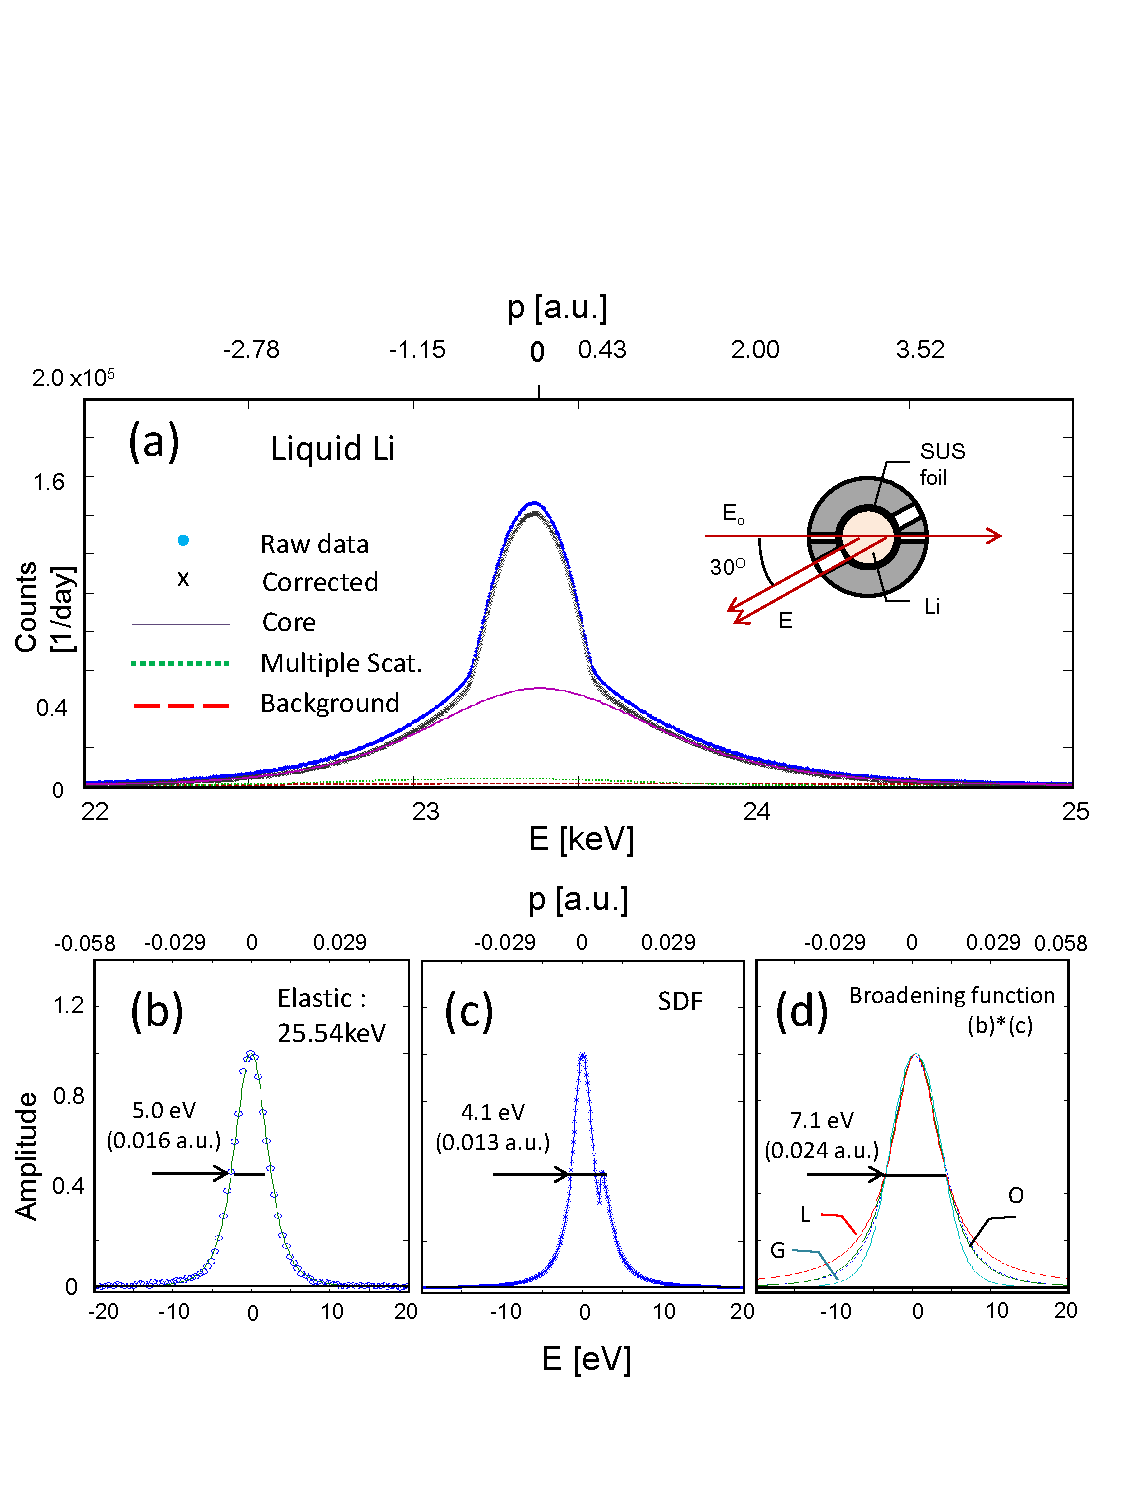
\includegraphics[bb= 30 50 500 600, width=7.5cm]{fig1.pdf}
\caption{(a) The CPs for liquid Li. The Inset shows the geometry of the experiment. (b) Elastic line, monitoring the instrumental resolution, 
(c) Spectral density function, indicating the final-state broadening, (d) The convolution of \small{(b)} and (c), providing the broadening function for a comparison with theory. O is the optimally fitted function while G and L denote Gaussian and Lorentzian, respectively.
} 
\label{Fig.1}
\end{figure}

%Among the elements, Na  is the closest to the HEG with nearly free electrons and an isotropic $n(k)$.
Lithium has been investigated as a case in which the HEG model is applicable.
However, there has been an unsolved puzzle for several decades.
Interacting HEG models generally predict $Z_{k_F}$ in the range 0.6-0.7 at Li valence density $r_s=3.25$.
The first experimental determination performed by Sch{\"u}lke \ii{et al.}\,provided 0.1$\pm$0.1 along the [100] axis based on a model analysis on $n(p)$ obtained \ii{via} a reconstruction on a single crystal~\cite{schulke96}.
In fact, there is a tendency %upon comparisons between theories and experiments in past decades (still true at present) 
for theory to predict higher CPs in $p<p_F$ while lower in $p>p_F$~\cite{saku95}.
Kubo~\cite{kubo95,kubo97} ascribed this to electron correlation effects, showing that his GW calculation agrees well with experiments and has a lower $Z_{k_F}$. He found it varies between 0.15-0.35 along several crystallographic axes.
Filippi and Ceperley calculated CPs by quantum Monte Carlo (QMC) simulation that explicitly includes electron-ion and electron-electron interactions, and concluded that electron correlation only partly accounted for the difference between theory and experiment~\cite{filippi99}.
Disorder~\cite{dugdale98} and temperature~\cite{stern01} were discussed as contributing to the difference but their analysis was not conclusive, leaving the puzzle unsolved.
Recently, Klevak \ii{et al.}~\cite{klevak16}, calculated EMD by a real-space multiple-scattering Green-function approach including disorder and found a smooth drop of $n(k)$ at $k_F$ with a very small $Z_{k_F}$. The results were similar to those of Kubo.
We note that the conduction electrons in Li have a strong orbital hybridization with core electrons, leading to a large electron-lattice interaction.
This renders the Fermi surface anisotropic and generates secondary Fermi surfaces in higher Brillouin zones due to the {\it{Umklapp}} process.
This makes quantitative comparisons between theory and experiment difficult. 

In this study, we estimate $Z_{k_F}$ in Li using ultra-high resolution Compton scattering. A 0.016 atomic unit (a.u.) instrumental resolution and a 0.024 a.u.\;overall resolution were achieved.
A tomographic reconstruction of the EMD is required for solid Li because it has an anisotropic Fermi surface. However, this reconstruction produces artifacts, making a quantitative analysis difficult.
To avoid this procedure, we measured Li above the melting point.
The liquid sample is isotropic, allowing a straightforward derivation of $n(k)$ from Eq. (2).
As a reference, we also measured a polycrystalline sample before melting the sample.
Both samples exhibit a clear break of $n(k)$ at $k_F$ allowing determination of the renormalization and the generic behavior of the momentum distribution of the HEG~\cite{holz11}.

\begin{figure}
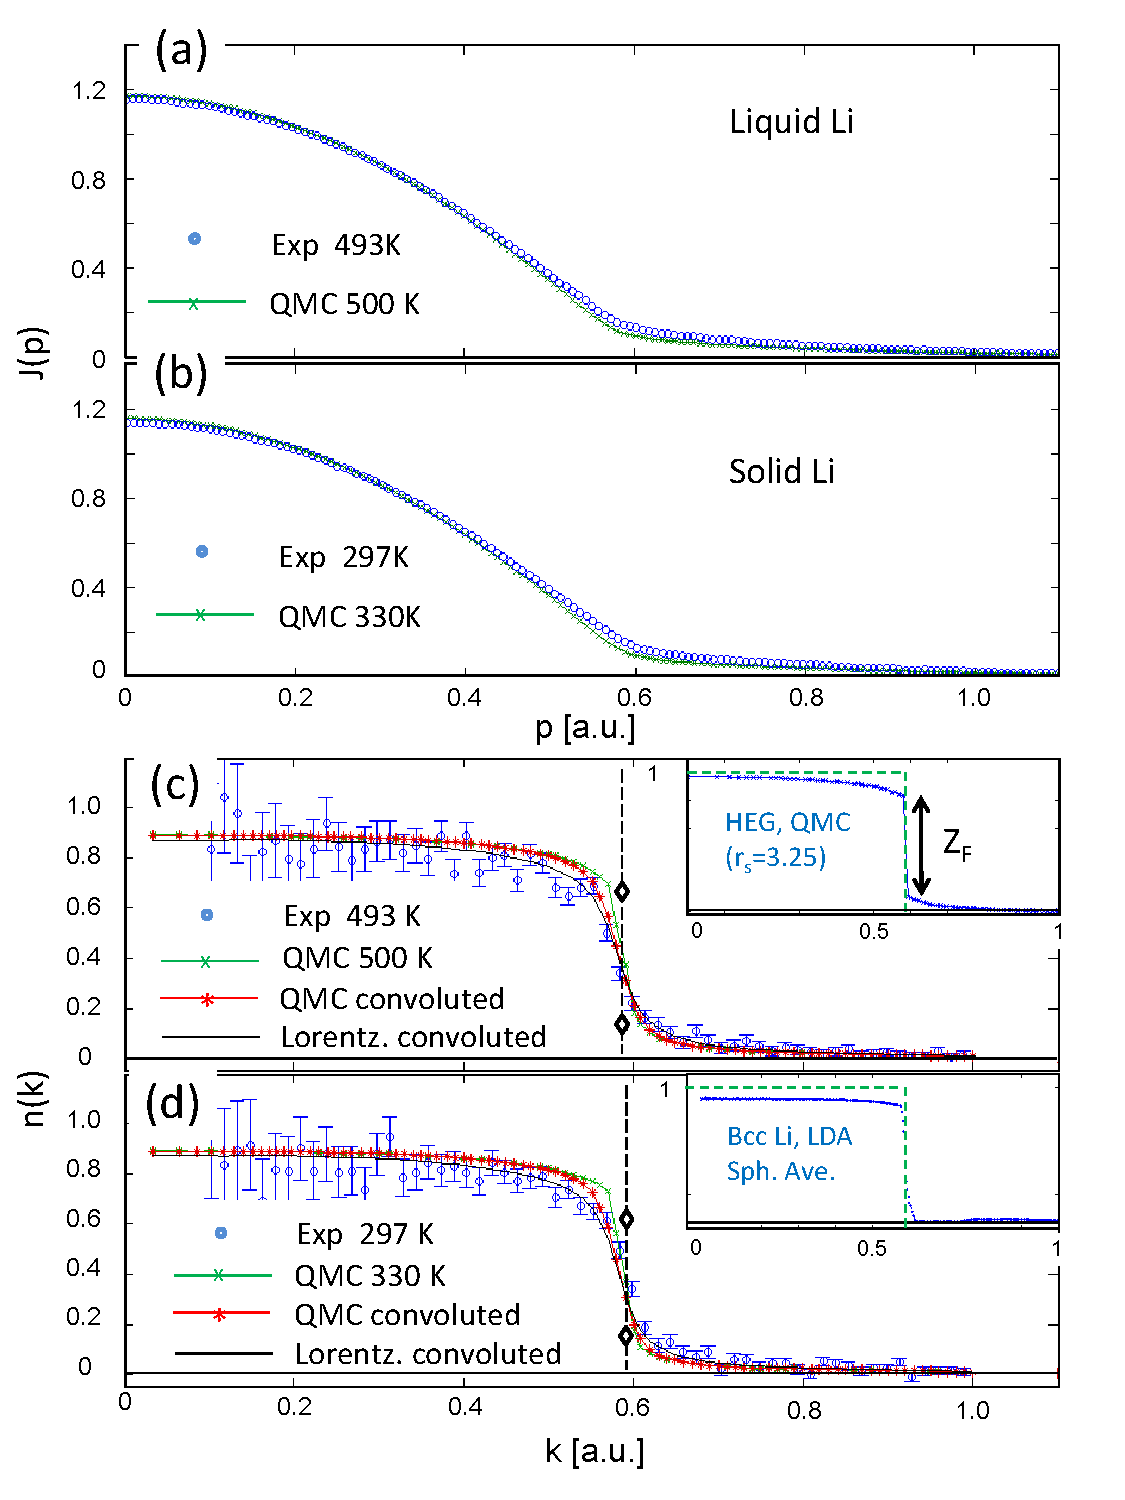
\includegraphics[bb= 50 10 500 720, width=7.5cm]{fig2.pdf}
\caption{CPs of liquid Li (a) and solid Li (b), compared with theory convoluted by the broadening function\dc{Can we add difference plots?}.  EMDs in liquid (c) and solid Li (d), compared to theory with or without the convolutions. The insets show EMD for HEG and the spherically averaged EMD from band theory (LDA). The $\Diamond$'s in (c) and (d)  show the $n(k_F)$ obtained by RPA fits near $k_F$.}
\label{Fig.2}
\end{figure}

The experiment was performed at Taiwan IXS beamline at SPring-8 (BL12XU).
The most critical parameter in determining $Z_{k_F}$ is the momentum resolution.
Since a typical radius of the Fermi sphere is 0.5 - 1.0\,a.u., a resolution of an order of 0.01\,a.u.\, is needed to estimate $Z_{k_F}$, which is a technical challenge.
One can easily improve the instrumental resolution if low energy photons are used but the spectrum is then substantially broadened by final-state effects~\cite{stern00,soi01}.
We have chosen $E_{\nn{\!o}}$=25.5 keV to obtain $dE$=5 eV (instrumental), corresponding to $dp$=0.016 a.u.
The details of the spectrometer are described in [\onlinecite{hira13}].

A polycrystalline Li sample having a cylindrical shape of 9-mm diameter and 10-mm height was placed in the furnace made of stainless steel (SUS) equipped with a heater at the bottom. See the inset in Fig.1a inset.
The experiment was first performed at 297 K on solid Li and then at 493 K on liquid Li.
The furnace had openings along the directions of the incident and the scattered photons (see, Fig.1a, inset).
The Li cylinder was rolled by a 10-$\mu$m thick SUS foil in a glovebox before setting \dc{???}, to avoid the sample spilling out of the furnace when melted.
As seen in the figure, the scattered photons from the foil were blocked by the thick part of the furnace so that they were not detected.
The obtained CPs were corrected for self-absorption, background, multiple scattering, and the energy dependence of the detection system (Fig.1a).

Diffusion Monte Carlo calculations were performed on molecular dynamics (MD) configurations of the ions sampled at 330K and 500K for the solid and the liquid phases, respectively. The classical MD temperatures were elevated by 33K in the solid and 7K in the liquid phase to account for quantum fluctuations of the nuclei by matching kinetic energy following ref.~\cite{filippi98}. We used Slater-Jastrow wavefunction with local density approximation (LDA) orbitals on simulation cells containing 432 lithium atoms. The finite-size error of the momentum distribution was corrected using the leading-order correction from Ref.~\cite{holz09}. The pseudopotential error was corrected using an all-electron calculation for the perfect crystal. All calculations were performed at $r_s=3.25$. After the QMC calculation, we rescaled $k$ and $n(k)$ to the $k_F$s corresponding to the actual experimental densities ($r_s=3.265$ for the solid and $r_s=3.31$ for the liquid). We used LAMMPS~\cite{Plimpton1993} for the MD simulations, QE~\cite{Giannozzi2009,Enkovaara2017} for the DFT calculations, and QMCPACK~\cite{Kim2018} for the QMC calculations. The disordered calculations have been automated using the Nexus suite of tools~\cite{Krogel2016}.
More computational details will be described elsewhere [cite theory paper].

\begin{table}[b]
\begin{tabular}{lllllll}
%\multicolumn{2}{l} {Averaging}   &      & $~n^-_{\nn{av}}~~~~$   & $~~n^+_{\nn{av}}~~~~$    & $~\zeta_{k_F}~~~~~$  & $Z_{k_F}$~   \\ \hline
%              & Theo. &\footnotesize{I}  & 0.76 & 0.077 & 0.69 & 0.83 \\
%Liquid    &      &\footnotesize{II} & 0.73 & 0.083 & 0.65& 0.78 \\
%              &      &\footnotesize{III}& 0.67 & 0.107 & 0.57 & 0.68 \\ % \hline
%              & Exp.  &      & 0.67 & 0.135 & 0.54 &  0.65 \\ \hline
%                            & Theo. &\footnotesize{I}~~~~  & 0.78~~~ & 0.065~~~ & 0.72~~~  & 0.86~~~ \\
%Solid      &           &\footnotesize{II} & 0.75 & 0.071 & 0.67  & 0.81 \\
%              &           &\footnotesize{III} & 0.69 & 0.098 & 0.59  & 0.71\\ %\hline
%              & Exp.  &      & 0.69 & 0.131 & 0.56 & 0.67 \\ \hline
%\\
\multicolumn{2}{l} {Power fit}    &  & $~n^-_{\nn{pow}}$     & $~n^+_{\nn{pow}}$      &   $\zeta_{k_F}$   &  $Z_{k_F}$    \\ \hline
              & Theo. &\footnotesize{QMC} & 0.74 & 0.091 & 0.65  & 0.78 \\
Liquid    &      &\footnotesize{QMC-C}& 0.73 & 0.091 & 0.64 &  0.77 \\
              &     &\footnotesize{QMC-CL} & 0.67 & 0.120 & 0.55 &  0.66 \\ % \hline
              & Exp.  &      & 0.69 & 0.142 & 0.54 & 0.62 \\ \hline
                  & Theo. &\footnotesize{QMC}  & 0.75 & 0.082 & 0.67 & 0.81 \\
Solid      &      &\footnotesize{QMC-C} & 0.74 & 0.084 & 0.66 & 0.80 \\
              &      &\footnotesize{QMC-CL} & 0.68 & 0.113 & 0.57 & 0.68 \\ % \hline
              & Exp.  &      & 0.72 & 0.144 & 0.57 & 0.65 \\ \hline
\\
\multicolumn{2}{l} {RPA fit}    &  & $~n^-_{\nn{RPA}}$     & $~n^+_{\nn{RPA}}$      &      &      \\ \hline
Liquid    & Theo. &\footnotesize{QMC} & 0.61 & 0.155 & 0.45 & \textbf{0.54} \\
Solid     & Theo. &\footnotesize{QMC} & 0.66 & 0.125 & 0.53 & \textbf{0.64} \\
\hline
\\
\multicolumn{3}{l} {RPA correction}    & $~n^-_{\nn{cor}}$     & $~n^+_{\nn{cor}}$      &      &      \\ \hline
              & Exp. &\footnotesize{QMC} & 0.56 & 0.206 & 0.35 &  0.42 \\
Liquid     &      &\footnotesize{QMC-C}& 0.57 & 0.206 & 0.36 & \textbf{0.43} \\
              &     &\footnotesize{QMC-CL} & 0.63 & 0.178 & 0.45 &  0.54 \\  \hline
              & Exp. &\footnotesize{QMC}  & 0.62 & 0.187 & 0.44 &  0.53 \\
Solid      &      &\footnotesize{QMC-C} & 0.63 & 0.185 & 0.45 & \textbf{0.54} \\
              &      &\footnotesize{QMC-CL} & 0.69 & 0.156 & 0.54 &  0.65 \\ % \hline
\hline\\
\end{tabular}
\caption{ \label{tab:zkf}
$Z_{k_F}$ and related parameters:
%``Averaging'' means the fit to $n(k)$ was determined by values of $k$ in the range:  $k_F-\delta k \le k \le k_F+\delta k$, where $\delta k=  0.05 a.u.$
``Power fit'' results are from a linear fit to $\ln(k)$ vs. $\ln(|k-k_F|)$.
``RPA fit'' means $n(k)$ is fitted to RPA form eq.~(\ref{eq:rpa-nk}).
``RPA  correction'' applies the correction $n^{\pm}_{\nn{cor}}$ =  $n^{\pm}_{\nn{pow}}$(Exp.)+$\Delta n^{\pm}$, where $\Delta n^{\pm}$ = $n^{\pm}_{\nn{RPA}}$(Theo.)-$n^{\pm}_{\nn{pow}}$(Theo.).Theory QMC are the raw  QMC $n(k)$ values, Theory QMC-C values are corrected with the convolution, and Theory QMC-CL are from the Lorentzian convolution having long tails.
\yy{The bold values are our best estimates.}
}
\end{table}

\begin{figure}
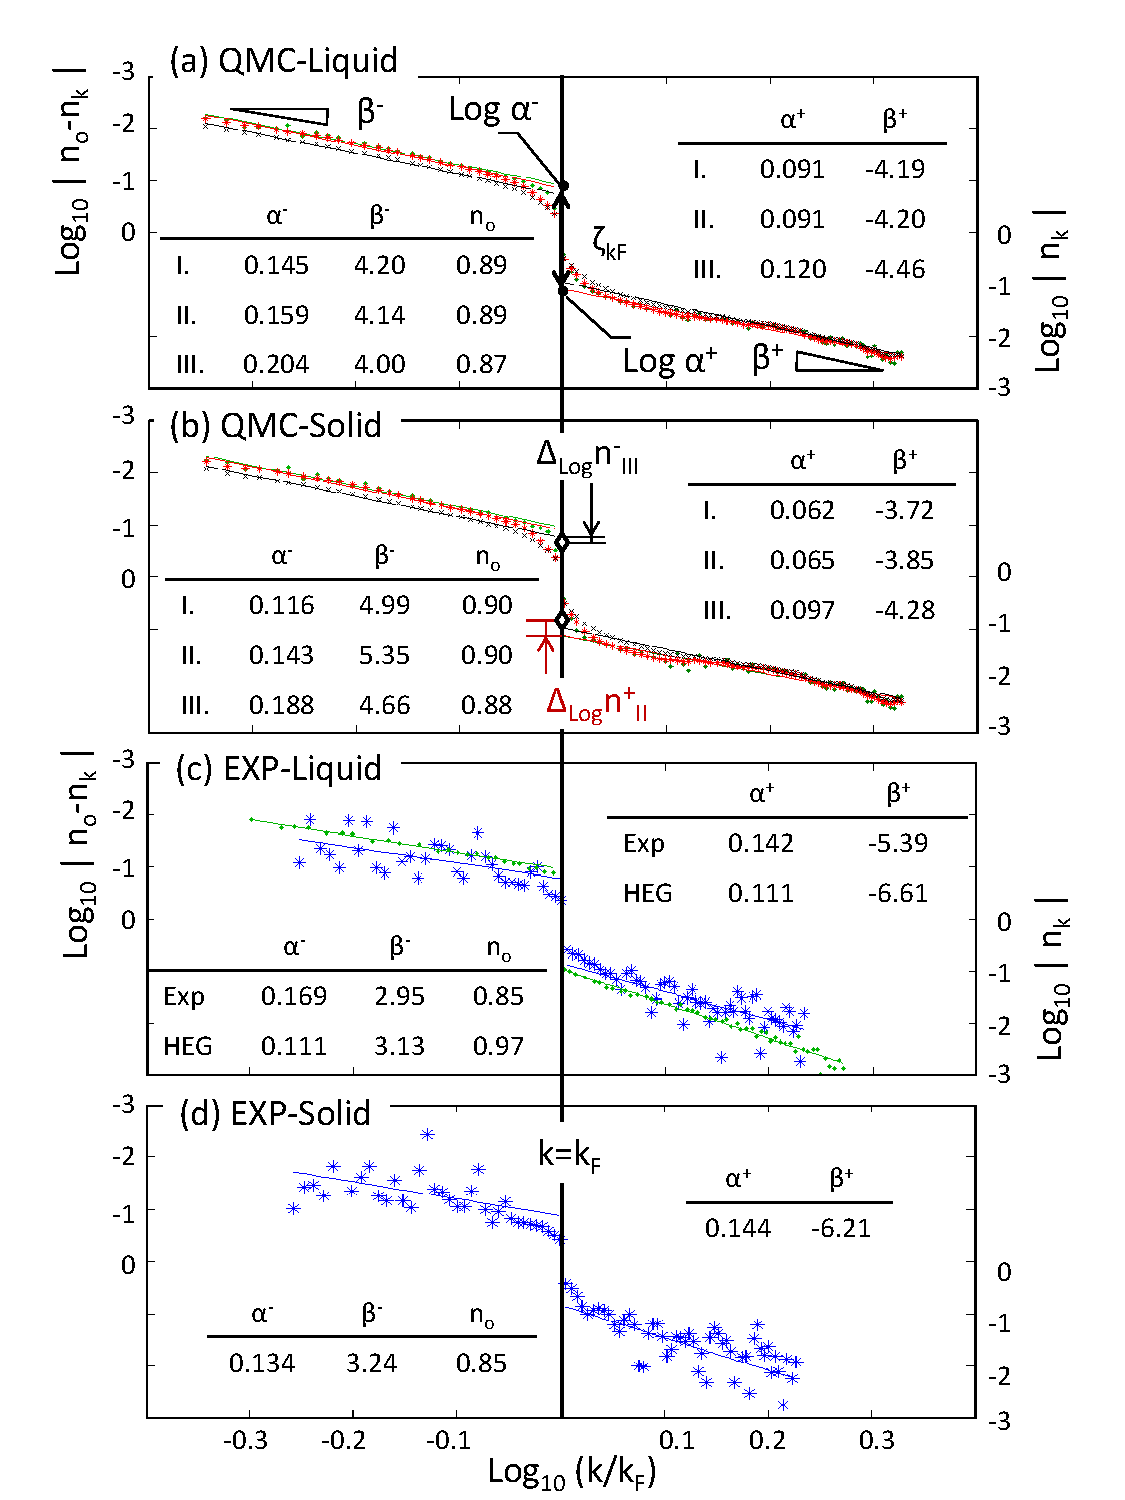
\includegraphics[bb= 70 10 500 700, width=7.5cm]{fig3.pdf}
\caption{Momentum densities vs. wave vector:  Theories for liquid (a) and solid (b) are shown. [$\cdot$] indicates original outputs (QMC), [$*$]  convoluted theory (-C), and [$\times$] convoluted with Lorentzian (-CL).  Experiments on liquid and solid are shown in (c) and (d). Those for HEG is also shown in (c).
 $\Diamond$ in (b) indicate $n^{\pm}$ by RPA fit ($n^{\pm}_{\nn{RPA}}$)  
while $\Delta_{\!\nn{Log}} n^{\pm}$ represents $ | \nn{log}_{10} n^{\pm}_{\nn{pow}} \,-\, \nn{log}_{10} n^{\pm}_{\nn{RPA}} | $,
where $ n^{\pm}_{\nn{pow}} $s are given by power fits for three cases \yy{(QMC, QMC-C, and QMC-CL)}.
} 
\label{Fig.3}
\end{figure}

Finally, theoretical CPs were convoluted by the broadening function due to the instrumental resolution and the final-state effect.
The former was monitored by a line profile of the elastic scattering (Fig.1b), which had a width of 0.016 a.u.
For the latter, we calculated a spectral density function (SDF) for HEG based on Soininnen's form~\cite{soi01}, which had a width of $\sim$ 0.013 a.u.\,(Fig.1c).
The broadening function given by a convolution of those functions showed a shape between Gaussian and Lorentzian.
We fit this profile with a broadening function $b(p) =1/ [ \Sigma_{n=0}^{2}\,a_n\,(2p / \Gamma )^{2n} ]$ and obtained ($a_0$, $a_1$, $a_2$) =(1.0, 0.85, 0.15) with $\Gamma$ = 0.024\,a.u.\,(Fig.1d).
Note this function becomes Lorentzian using the parameters (1, 1, 0) while effectively Gaussian using the parameters (0.6, 0.3, 0.1).

Figure 2a compares the experimental (valence) CPs, $J(p)$, to theory (convoluted) while Fig.2b the experimental $n(k)$s to theory with and without convolutions.
As a reference, another $n(k)$ convoluted by Lorentzian having longer tails is also shown.
We first computed  $J(p)$ with Eq.(1), then convoluted, and then transformed back to $n(k)$ with Eq. (2).
$n(k)$s of the liquid and solid Li are similar and clear features of the momentum distribution renormalization can be seen.
Theory seems to match the experiment better with the Lorentzian-type broadening function, especially the height of $n(k)$ and the curvature near $k_F$, perhaps implying that SDF could have a larger tail than expected.
This possibility will be discussed later.
Liquid Li has a slightly lower density, thus a smaller $k_F$, making $J(p)$ higher for $k < k_F$.
Furthermore, $n(k)$ in the liquid shows a slightly smaller drop at $ k_F $  possibly because of more disorder effect and  larger electron correlation effect in the expanded system.
As mentioned above, solid Li has an anisotropic Fermi surface; its radius varies by several percent~\cite{saku95,schulke96}. Hence a simple comparison is problematic.
Nonetheless, the comparison across the melting point is consistent with expectations, indicating that the solid sample consists of randomly oriented domains.
A sharp drop at $k_F$ persists even after the spherical averaging, as we verified with band theory calculations based on the LDA (see, Inset in Fig.2d).

%In order to determine $Z_{k_F}$ we follow the procedure in earlier study of Na~\cite{simo10}: $Z_{k_F}$ is determined by the difference between $dJ/dp$ at $p\,$s slightly smaller and larger than $p_F$.
%This is equivalent to evaluating the difference between $n(k)$ at $k\,$s slightly smaller and larger than $k_F$.
%Once one has $n^+$ and $n^-$ by averaging $n(k)$\,s among several points near $k_F-\delta k$ and  $k_F+\delta k$, respectively, the difference $\zeta_{k_F}$ = $n^- - n^+$ provides the gap.
%Note that this renormalization factor that is reduced due to electron-lattice interaction, thus
%$Z_{k_F}$ is given by $\zeta_{k_F}/n_{k_F}^{\nn{DFT}}$~\footnote{this ratio is double-checked by LDA band-theory, where $n_{k_F}$=0.83 for bcc Li.}.
%$n_{k_F}^{\nn{DFT}}$ is the DFT momentum distribution just inside the Fermi surface ($\approx$0.83), which accounts for electron-lattice interaction.
%The obtained $Z_{k_F}\,$s are summarized in the ``Averaging'' section of TABLE~\ref{tab:zkf}.

%The advantage of the above analysis is that it is independent of the model but it obviously tends to overestimate $Z_{k_F}$ as the momentum densities are determined away from $k_F$.
$Z_{k_F}$ is defined in the limit of $k$ $\to$ $k_F$.
Sch{\"u}lke \ii{et al.}\,\,constructed a model where $n(k)$ decreases as $-(k/k_F)^{8}$ or $(k/k_F)^{-8}$ with increasing $k$~\cite{schulke96}.
Based on their model, we first tried to plot $n(k)$ $vs$ $(k/k_F)^{\pm 8}$ but we did not find a linear behavior.
%This fact encourages us to carefully investigate the asymptotic behaviors upon 
We assume a more general power law behavior:
\begin{eqnarray}
n(k) &=& n_0 - \alpha^{-}  (k/k_F)^{\beta^-}  \;\;\;\; (k \leq k_F)  \nonumber \\
&=&  \alpha^{+}  (k/k_F)^{\beta^+}  \;\;\;\;\;\;\;\;\;\;\;\; (k>k_F).
\end{eqnarray}
%Here, $\alpha^{+(-)}$ indicate the densities extrapolated at ${k=0\,(\infty) \to k_F}$ and $\beta^{+(-)}$ the exponent.
The $-$ (or $+$) sign represents the extrapolation from below (or above) $k_F$.

Figure 3 shows the log-log plots for $n(k)$ vs $(k/k_F)$. %, on which linear fits are indicated together. 
We find that the theoretical $n(k)$ has  exponents $\beta$$\sim\pm$4, depending on the broadening functions.
The HEG  would have $\beta$ = -8 at $k \gg k_F$, which is very different from the results for Li.
The reasons for the difference is (i) that HEG can have a different behavior as $k$ approaches $k_F$ and (ii) that {\it Umklapp} process may significantly influence the asymptotic behavior.
The experiments, on the other hand, shows $\beta^+$$\sim\,$3 and $\beta^-$$\sim\,$-5.
The non-negligible difference between theory and experiment may be due to {\it Umklapp} features that appear more prominent in theory.
%It is noted that, if the average was taken for the absolutes $| \beta^+ |$ and $| \beta^- |$, it would be 4$\sim$5, which agrees with theory.
%This exponent may be a characteristic parameter describing behaviors in a practical $k$ range.
%Now we determine $Z_{k_F}$s. 
The extrapolated densities $\alpha^-$ and $\alpha^+$ give $n_o - n^-$ and $n^+$, respectively.
$Z_{k_F}$ is given by $\zeta_{k_F} (n_{k_F}^{\nn{FFG}}/n_{k_F}^{\nn{DFT}})$, where $\zeta_{k_F}= n^- - n^+$.
The renormalization factors $Z_{k_F}$s are summarized in %the ``Power fit'' section of 
Table~\ref{tab:zkf}.
%TABLE~\ref{tab:zkf} summarizes the ${\color{black}Z_{k_F}}$s. 
%The theory originally provides $Z_F$ = 0.76 for liquid and 0.78 solid  (see, Theory-I in TABLE~\ref{tab:zkf}) .
%They are diminished to 0.74 and 0.76 after the convolution by $b(p)$ (Theory-II), meaning the experimentally observed ${\color{black}\zeta_{k_F}}$ requires the correction for this, which amounts to 2.8 \%.
%The experimental ${\color{black}Z_{k_F}}\,$s are 0.62 (L) and 0.65 (S). After the corrections, we have ${\color{black}Z_{k_F}}\,$s = 0.64 (L) and 0.67 (S) at the end.    

The power model fits given as Eq.\,(3) tend to overestimate $Z_{k_F}$ because the momentum distribution is expected to have a divergent slope at $k_F$~\cite{gg02}.
This effect is significant in Li though such a deviation is much smaller in HEG [see, Fig.3(c)].
To account for the slope, we fit the QMC $n(k)$ to the RPA form Eq.~(\ref{eq:rpa-nk})
\begin{equation} \label{eq:rpa-nk}
\tilde{n}(x) = n_1 + A\vert 1-x\vert log\left(\vert 1-x\vert\right),
\end{equation}
where $x\equiv k/k_F$, $\tilde{n}\in[0,1]$. $n_1$ and $A$ are fitting parameters. The fitted $n_1$ corresponds to $n^-$ in the range $x\in(0.8, 0.97)$ and $n^+$ in the range $x\in(1.02, 1.2)$. Points too close to $k_F$ were excluded because spherical average of anisotropic $n(\boldsymbol{k})$ smears out the Fermi break. $k_F$ of the MD configurations were determined by unfolding the LDA bands from the 432-atom supercell to the primitive cell Brillouin zone using the BandUP code~\cite{Medeiros2014,Medeiros2015}. $Z_{k_F} = \langle\zeta_{k_F}\rangle/n_{k_F}^{\nn{LDA}}$, where
$\langle\rangle$ indicates average over MD configurations and
$n_{k_F}^\nn{LDA}\approx0.83$. The QMC $Z_{k_F}$ obtained in this way are
$0.64\pm0.01$ and $0.54\pm0.01$
for the solid and liquid, respectively.

The RPA form Eq.~(\ref{eq:rpa-nk}) cannot be directly fit to the experimental data because of resolution and final-state smearing effects at $k_F$.
Therefore, we use theory to determine the slope near $k_F$ and attempt to correct the experimental $\zeta_{k_F}$ and $Z_{k_F}$ based on the theoretical slope.
The difference between the extrapolated densities in the two models $\Delta n^{\pm}$ $\equiv$ $n^{\pm}_{\nn{pow}} (theo.)$$-$$n^{\pm}_{\nn{RPA}}$ are exploited for the corrections to the experiments.
$\Delta n^{\pm}$ depends on a shape of the broadening function $b(p)$, which involves the SDF that is not entirely clear \yy{which may not be exact} (see, Table~\ref{tab:zkf}) and leads to an uncertainly for determining $Z_{k_F}$.
The experimental $n^{\pm}$s, $\zeta_{k_F}$s, and $Z_{k_F}$s after the corrections are shown in the last rows of Table~\ref{tab:zkf}.
Assuming the behavior of the  QMC determined $n(k)$ for values k suchd that $k ~ k_F$, an upper estimate for $Z_{k_F}$ is  0.54 (liquid) and 0.65 (solid) by the broadest, Lorentzian-type $b(p)$ while the lower estimates are 0.42 (liquid) and 0.53 (solid) by the narrowest $b(p)$.
In summary, we obtained in experiment $Z_{k_F}=  0.43^{\nn{+0.11}}_{\nn{\;-0.01}}$ for liquid Li and 0.54$^{\nn{+0.11}}_{\nn{\;-0.02}}$ for solid Li, while using QMC we obtained $0.54\pm0.01$ for the liquid and $0.64\pm0.01$ for the solid.
The agreement is much better than in previous studies.
To reduce the experimental errors further, the broadening due to final state effects needs to be made smaller by Compton scattering at higher energies, {\it{e.g.}} at $\sim$50 keV.
%while theoretical ones by QMC are {\color{red}0.54$\pm0.01$(L) and 0.64$\pm0.01$(S)}.
%They agree with each other, much more reasonably compared to the earlier reports.% having posted many disputes.   


%The log-log fits tend to overestimate $Z_{k_F}$ because the momentum distribution is expected to have a divergent slope at $k_F$~\cite{gg02}. To account for this slope, we fit the QMC $n(k)$ to the RPA form eq.~(\ref{eq:rpa-nk})
%\begin{equation} \label{eq:rpa-nk}
%\tilde{n}(x) = n_1 + A\vert 1-x\vert log\left(\vert 1-x\vert\right),
%\end{equation}
%where $x\equiv k/k_F$, $\tilde{n}\in[0,1]$. $n_1$ and $A$ are fitting parameters. The fitted $n_1$ corresponds to $n^+$ in the range $x\in(0.8, 0.97)$ and $n^-$ in the range $x\in(1.02, 1.2)$. Points too close to $k_F$ were excluded because spherical average of anisotropic $n(\boldsymbol{k})$ smears out the Fermi break. $k_F$ of the MD configurations were determined by unfolding the LDA bands from the 432-atom supercell to the primitive cell Brillouin zone using the BandUP code~\cite{Medeiros2014,Medeiros2015}. The $n(k)$ discontinuity $\zeta_{k_F}= \langle n^+-n^-\rangle$, where $\langle\rangle$ indicates average over MD configurations. Finally, $Z_{k_F} = \zeta_{k_F}/n_{k_F}^{LDA}$, where $n_{k_F}^{LDA}\approx0.83$. The QMC $\zeta_{k_F}$ obtained in this way are $0.53\pm0.01$ and $0.45\pm0.01$ for the solid and liquid, respectively. The $Z_{k_F}$s are $0.64\pm0.01$ and $0.54\pm0.01$.
%The RPA form eq.~(\ref{eq:rpa-nk}) cannot be straight-forwardly fit to the experimental data due to resolution and final-state smearing effects at $k_F$. The good agreement between QMC and experiment away from $k_F$ is support for our QMC $Z_{k_F}$ results.
%
%\vspace{10mm}
%
%Finally we evaluate the error bars on our experimental outputs.
%The main errors arise from uncertainty of SDF for the final state.
%The experimental ${\color{black}Z_{k_F}}$ are commonly smaller than those for the theory.
%This could be due to SDF perhaps having a longer tail than we exact, just like Lorentzian (Theory-III). 
%If this is the case, the correction would have to be as large as 18 \%, to estimate the originals, and thus the experimental ${\color{black}Z_{k_F}}$s would be significantly larger, 0.75 (L) and 0.79(S) after the correction. 
%They can be considered as the upper limits.
%The lower limits would be estimated when $\delta$-function used as SDF. This correction is much smaller, only 2\% at most (not shown).
%We then have 0.63(L) and 0.66(S) after the corrections as the lowest limit.    
%
%In summary,  the experimental ${\color{black}Z_{k_F}}$s with errors are 0.64$^{\nn{+0.11}}_{\nn{\;-0.01}}$ for liquid Li and 0.67$^{\nn{+0.12}}_{\nn{\;-0.01}}$ for solid, %while theoretical ones by QMC are 0.76 (L) and 0.78 (S).
%while theoretical ones by QMC are {\color{red}0.54$\pm0.01$(L) and 0.64$\pm0.01$(S)}.
%They agree with each other, much more reasonably compared to the earlier reports.% having posted many disputes.      



The experiment was performed under approvals of JASRI/SPring-8 (Prop. No. 2011B4250, 2012A4253-4254) and NSRRC, Taiwan (2011-2-105).
DC and YY were supported by DOE Grant NA DE-NA0001789.
\yy{This work made use of the Blue Waters sustained-petascale computing project and the Illinois Campus Cluster, supported by the National Science Foundation (awards OCI-0725070 and ACI-1238993), the state of Illinois, the University of Illinois at Urbana-Champaign and its National Center for Supercomputing Applications.}
       
\bibliography{lithium}
%\begin{thebibliography}{2}
%\expandafter\ifx\csname natexlab\endcsname\relax\def\natexlab#1{#1}\fi
%\expandafter\ifx\csname bibnamefont\endcsname\relax
%  \def\bibnamefont#1{#1}\fi
%\expandafter\ifx\csname bibfnamefont\endcsname\relax
%  \def\bibfnamefont#1{#1}\fi
%\expandafter\ifx\csname citenamefont\endcsname\relax
%  \def\citenamefont#1{#1}\fi
%\expandafter\ifx\csname url\endcsname\relax
%  \def\url#1{\texttt{#1}}\fi
%\expandafter\ifx\csname urlprefix\endcsname\relax\def\urlprefix{URL }\fi
%\providecommand{\bibinfo}[2]{#2}
%\providecommand{\eprint}[2][]{\url{#2}}
%
%\bibitem[{\citenamefont{Erskine and Stern}(1975)}]{erskine75}
%\bibinfo{author}{\bibfnamefont{J.~L.} \bibnamefont{Erskine}} \bibnamefont{and}
%  \bibinfo{author}{\bibfnamefont{E.~A.} \bibnamefont{Stern}},
%  \bibinfo{journal}{Phys. Rev. B} \textbf{\bibinfo{volume}{12}},
%  \bibinfo{pages}{5016} (\bibinfo{year}{1975}).
%
%\bibitem[{\citenamefont{Sch{\"u}tz et~al.}(1987)\citenamefont{Sch{\"u}tz,
%  Wagner, Wilhelm, Kienle, Zeller, Frahm, and Materlik}}]{schutz87}
%\bibinfo{author}{\bibfnamefont{G.}~\bibnamefont{Sch{\"u}tz}},
%  \bibinfo{author}{\bibfnamefont{W.}~\bibnamefont{Wagner}},
%  \bibinfo{author}{\bibfnamefont{W.}~\bibnamefont{Wilhelm}},
%  \bibinfo{author}{\bibfnamefont{P.}~\bibnamefont{Kienle}},
%  \bibinfo{author}{\bibfnamefont{R.}~\bibnamefont{Zeller}},
%  \bibinfo{author}{\bibfnamefont{R.}~\bibnamefont{Frahm}}, \bibnamefont{and}
%  \bibinfo{author}{\bibfnamefont{G.}~\bibnamefont{Materlik}},
%  \bibinfo{journal}{Phys. Rev. Lett.} \textbf{\bibinfo{volume}{58}},
%  \bibinfo{pages}{737} (\bibinfo{year}{1987}).



%\end{thebibliography}


\end{document} 




   


     
     
 
   

 

